\documentclass[12pt,a4paper]{article}
\usepackage[utf8]{inputenc}
\usepackage[spanish]{babel}
\usepackage[T1]{fontenc}
\usepackage{tocbibind} % Bibliografía en el indice
\usepackage{titlesec} % Posibilidad de editar los formatos de chapter
\usepackage{amsmath,amssymb,mathrsfs} % Matemáticas varias
\usepackage{siunitx} % SI de medidas
\usepackage{tabularx} % Para las tablas
\usepackage[title]{appendix} % Para anexos
\usepackage[spanish]{babel} % Para modificar labels por defecto
\renewcommand{\baselinestretch}{1} % Interlineado. 1 es estandar
% --- Arreglos varios para la inclusion de imagenes
\usepackage{float}
\usepackage[pdftex]{graphicx}
\usepackage{subfigure}
\usepackage{graphicx}
\graphicspath{{T:/Tom/Facultad/Logos/}{T:/Tom/Facultad/Materias/EDII/TPs/LED/Imagenes/}}
\usepackage[usenames,dvipsnames]{color}
\DeclareGraphicsExtensions{.png,.jpg,.pdf,.mps,.gif,.bmp}
% --- Para las dimensiones de los márgenes etc
\frenchspacing \addtolength{\hoffset}{-1.5cm}
\addtolength{\textwidth}{3cm} \addtolength{\voffset}{-2.5cm}
\addtolength{\textheight}{4cm}
% --- Para el encabezado
\setlength{\headheight}{33pt}
\usepackage{fancyhdr}
\fancyhead[R]{\includegraphics[height=1cm]{logo_fcefyn_nuevo.jpg}}\fancyhead[L]{\includegraphics[height=1cm]{unc1_a.jpg}}\fancyhead[C]{Electrónica Digital II} \fancyfoot[C]{Página \thepage} \renewcommand{\footrulewidth}{0.4pt}
\pagestyle{fancy}
% --- Para las tablas
\usepackage{multirow} % Juntar filas
\newcolumntype{L}[1]{>{\raggedright\arraybackslash}p{#1}} % Justificar Izq
\newcolumntype{C}[1]{>{\centering\arraybackslash}p{#1}} % Justificar Centrar
\newcolumntype{R}[1]{>{\raggedleft\arraybackslash}p{#1}} % Justificar Der
\usepackage[numbered]{bookmark} % Para que figure las secciones en el PDF
\usepackage{listings} % Para poner código 
\usepackage{enumitem} % Para editar las propiedades de los items
\usepackage{color}
\usepackage[bottom]{footmisc} % Para las notas al pie de la página
\lstset{frame=single} % Código en un cuadro
% --- Para Anexo
\addto\captionsspanish{%
  \renewcommand\appendixname{ANEXO}
  \renewcommand\appendixpagename{ANEXOS}
}
% -------------------------------------------------------- %
% Definicion de colores para el codigo
\lstdefinelanguage{XML}
{
  basicstyle=\ttfamily\footnotesize,
  morestring=[b]",
  moredelim=[s][\bfseries\color{Maroon}]{<}{\ },
  moredelim=[s][\bfseries\color{Maroon}]{</}{>},
  moredelim=[l][\bfseries\color{Maroon}]{/>},
  moredelim=[l][\bfseries\color{Maroon}]{>},
  morecomment=[s]{<?}{?>},
  morecomment=[s]{<!--}{-->},
  commentstyle=\color{DarkOliveGreen},
  stringstyle=\color{blue},
  identifierstyle=\color{red}
}

\renewcommand{\lstlistingname}{Código}

% -------------------------------------------------------- %

\begin{document}

\begin{titlepage}
    \begin{center}
        \vspace*{1cm}
        
        \Large
        \textbf{Universidad Nacional de Córdoba\\
        		Facultad de Ciencias Exatas, Físicas y Naturales}
        
        \vspace{0.5cm}
        \includegraphics[width=0.5\textwidth]{logo_caratula.png}
        
        \vspace{1.5cm}
        
        \textbf{Primer Trabajo Práctico}\\
        Electrónica Digital II\\
        Docente: Ing. Martín Del Barco
        
        \vfill  
        
        \vspace{0.8cm}
        

        
        \Large
        Losano Quintana, Juan Cruz\\
        Piñero, Tomás Santiago\\
        Ingeniería en Computación\\
        Año 2019\\
        
        
    \end{center}
\end{titlepage}
% -------------------------------------------------------- %

% --- Tabla de contenidos

\setcounter{secnumdepth}{1}
\setcounter{tocdepth}{4}
\tableofcontents

% -------------------------------------------------------- %

\newpage
\renewcommand{\baselinestretch}{1}
\setlength{\parskip}{0.5em}

\section{Enunciado}
	Realizar un programa que permita sumar dos valores de cuatro bits cada uno, ingresados desde puertos configurados como entradas. El resultado debe mostrarse mediante cuatro LEDs conectados a puertos configurados como salidas. En caso de producirse un acarreo del tipo ``\emph{Digit Carry}'', un quinto LED empezará a parpadear indefinidamente con un periodo de aproximadamente un segundo prendido y un segundo apagado. A partir de ese instante ya no podrán realizarse más sumas, salvo que se realice un reset del microcontrolador.
	
	Armar en la protoboard el circuito totalmente funcional para ser presentado y evaluado en clase.
	
	Adjuntar una foto de la hoja que muestre el diagrama de todas las conexiones realizadas en el diseño con el cálculo del valor de las resistencias limitadoras de los puertos de salida y el cálculo del tiempo de parpadeo de los bucles anidados utilizados para la frecuencia de reloj elegida.

\newpage

\section{Introducción}
	Para la realización del trabajo práctico se utilizaron los siguientes materiales:
	
	\begin{itemize}[leftmargin=1.5cm,nosep]
	\item Microcontrolador PIC16F887.
	\item Cristal de \SI{4}{\MHz}.
	\item LEDs de color verde, amarillo y rojo.
	\item Resistencias de \SI{1}{\kilo\ohm}, \SI{330}{\ohm} y \SI{220}{\ohm}.
	\item Capacitores de \SI{22}{\pico\F} y \SI{100}{\nano\F}.
	\item Dos Dip Switch (DS) de cuatro llaves.
	\item Un pulsador.
	\end{itemize}

	Al ser dos números de cuatro bits, el resultado será de cinco bits en el peor de los casos, por lo tanto se pueden utilizar dos puertos del PIC para implementar el circuito, ya  que éste posee cuatro puertos de ocho bits.
	
	Se seleccionó el puerto B como puerto de entrada de ambos números y el puerto A como salida para mostrar el resultado de su suma.

\section{Desarrollo}
\subsection{Cálculos de resistencias}
	Antes de realizar la implementación del circuito se deben calcular las resistencias para las salidas del PIC.
	
\subsubsection{Pull-ups}
	Las resistencias \emph{pull-up} son utilizadas en circuitos digitales para asegurar en cualquier circunstancia un nivel lógico seguro y definido en una determinada entrada o pin digital. Los estados lógicos son tres:

\begin{enumerate}[leftmargin=1.5cm,nosep]
\item Alto (\emph{High}): también llamado \emph{uno lógico}, representa la presencia de voltaje.
\item Bajo (\emph{Low}): también llamado \emph{cero lógico}, representa la ausencia de voltaje.
\item Flotante (\emph{Floating}): estado de \emph{alta impedancia}, desconectado del resto del circuito.
\end{enumerate}
	
	 Las resistencias pull-up se utilizaron para el pulsador de reset.	
	
	\paragraph{Reset}
	En este caso las resistencias cumplen una doble función:
	\begin{enumerate}[leftmargin=1.5cm,nosep]
	\item Limitar la corriente en el pin.
	\item Impide la conexión directa del pin a $V_{cc}$ cuando se presiona el pulsador, evitando así un cortocircuito.
	\end{enumerate}
	
	Se utilizó el circuito recomendado en hoja de datos del PIC para el \emph{Master Clear} ($\overline{MCLR}$) en la sección 14 \emph{Special Features of the CPU}, subsección 2.1 \emph{Power-on Reset (POR)}, página 213.
	
	\begin{figure}[h]
	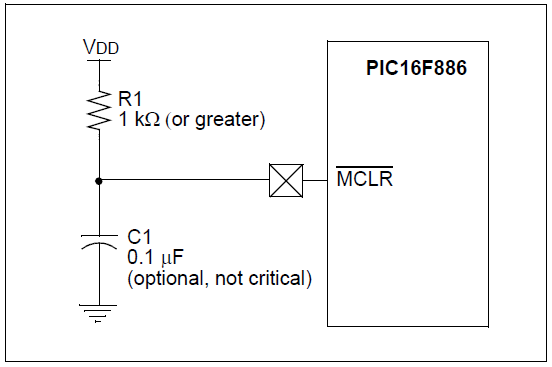
\includegraphics[scale=0.6]{reset.png}
	\centering
	\caption{Circuito recomendado para el $\overline{MCLR}$}
	\end{figure}
	
	\paragraph{Puerto de entrada}
	Se eligió el puerto B como entrada debido a que es el único de los cinco puertos que tiene pull-up integrado, evitando así el cálculo e implementación de resistencias adicionales. 
	
	Estos pull-up internos deben habilitarse vía software desde el bit siete (\emph{$\overline{RBPU}$}) del registro de opciones (\emph{OPTION\textunderscore REG}) y configurarse por medio del registro \emph{WPUB}.
	
\subsubsection{LEDs}
	Las resistencias para cada LEDs se calculan según la \emph{Ley de Ohm} y teniendo en cuenta la tensión máxima de salida del puerto en alto $V_{OH}$. Según la hoja de datos,  este valor de tensión es de $V_{cc}-0.7 V$ (ver sección 17 \emph{Electrical Specifications}, subsección 5 \emph{DC Characteristics}, página 251).
	
	Como el circuito se alimenta con \SI{5}{\V}, el valor será $V = V_{OH} = 4.3 V$. Por lo tanto el circuito para los LEDs queda de la siguiente manera:
	
	\begin{figure}[h]
	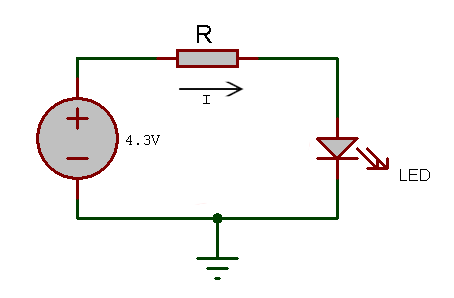
\includegraphics[width=8cm]{LED.png}
	\centering
	\caption{Circuito LED}
	\label{fig:leds}
	\end{figure}		
	
	\newpage
	La corriente I de la Figura \textbf{\ref{fig:leds}} deseada para cada LED es de \SI{10}{\mA}, por ende las ecuaciones quedan:
	
	\begin{align*}
	4.3 V &= V_{LED} + V_{R} \\
	4.3 V &= V_{LED} + I * R \\
	4.3 V &= V_{LED} + 10 mA * R \\
	\end{align*} 
	 
	\begin{align} \label{res}
	R &= \frac{4.3 V - V_{LED}}{10 mA}  
	\end{align}
	
	El valor de las resistencias que se pondrán como resultado es el normalizado, redondeado, en lugar del calculado.
	
	\paragraph{LED Rojo}
	El LED de color rojo se activa con una tensión de \SI{1.7}{\V}, por lo tanto, la ecuación \textbf{\ref{res}} queda:
	
	\begin{align*}
	R &= \frac{4.3 V - 1.7 V}{10 mA}  
	\end{align*}
		
	\begin{align}
	R &=  \SI{330}{\ohm}
	\end{align}	
	
	\paragraph{LED Verde}
	El LED de color verde se activa con una tensión de \SI{2.2}{\V}, por lo tanto, la ecuación \textbf{\ref{res}} queda:
	
	\begin{align*}
	R &= \frac{4.3 V - 2.2 V}{10 mA}  
	\end{align*}
	
	\begin{align}
	R &=  \SI{220}{\ohm}
	\end{align}	
	
	

\newpage
\section{Implementación}
	El PIC tiene como frecuencia de reloj un cristal de \SI{4}{\MHz}, por lo que el ciclo de instrucción se realiza con una frecuencia de \SI{1}{\MHz} debido a que cada 4 ciclos del reloj se realiza una instrucción. Esto se debe a que para ejecutar la instrucción indicada, el PIC debe ejecutar cuatro acciones: 
	
	\begin{enumerate}[leftmargin=1.5cm,nosep]
	\item Buscar la instrucción en la memoria principal.
	\item Decodificar la instrucción.
	\item Ejecutar la instrucción.
	\item Almacenar los resultados.
	\end{enumerate}
	
	Esto es importante para el cálculo de la subrutina de retardo, ya que depende de la frecuencia de reloj que se utilice.
	
	A continuación se muestran los diagramas de flujo del programa utilizado.
	
\subsection{Diagramas de flujo}
	En esta sección se muestran los diagramas de flujo del programa principal y las subrutinas que utiliza.
	
	\subsubsection{Programa principal}	
	Primero se realiza la configuración de los puertos A y B como salida y entrada digitales, respectivamente. 
	
	Una vez configurados los puertos se toman los datos del puerto de entrada y a esa lectura se la invierte, ya que cuando los Dip Switch estén bajos las entradas estarán con un valor de uno lógico debido a la presencia de las resistencias pull-up.
	
	Consecuentemente el programa almacena los últimos cuatro bits en la variable \emph{numero1} y se lo suma a los primeros cuatro bits leídos, mostrando el resultado en los LEDs de salida. Si el resultado es de cinco bits, el LED del \emph{digit carry} parpadeará y no se podrá realizar otra suma hasta que se resetee el PIC.
	
	\begin{figure}[H]
	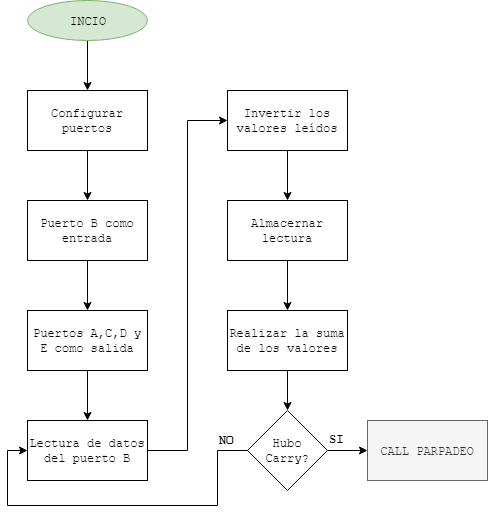
\includegraphics[scale=0.5]{programa.png}
	\centering
	\caption{Diagrama de flujo del programa.}
	\end{figure}		
	
	\subsubsection{Parpadeo}
	Es una subrutina muy simple que se encarga solamente de encender y apagar el LED correspondiente al \emph{digit carry} con un retardo de aproximadamente un segundo.
	
	\begin{figure}[H]
	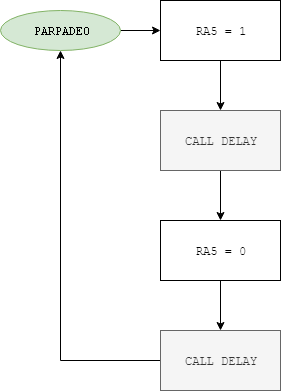
\includegraphics[scale=0.5]{parpadeo.png}
	\centering
	\caption{Diagrama de flujo de la subrutina \emph{Parpadeo}.}
	\end{figure}		
	
	\newpage
	\subsubsection{Delay}
	Como se mecionó anteriormente, esta subrutina demora aproximadamente un segundo en ejecutarse, por lo que se utiliza para el parpadeo del \emph{digit carry}.
	
	El cálculo para su realización es el siguiente:
	
	\begin{align*}
	\SI{4}{\micro \second} * (cuenta - \SI{1}{\micro \second}) + \SI{5}{\micro \second} &=  \SI{1000000}{\micro \second} \\
	cuenta &= \frac{\SI{1000000}{\micro \second}}{\SI{4}{\micro \second}} - \SI{4}{\micro \second}
	\end{align*}
	
	\begin{align}
	cuenta &= 249996
	\end{align}
	
	Al ser registros de ocho bits, un contador solamente puede llegar hasta 256, por lo que para llegar al valor de \emph{cuenta} calculado se utilizarán tres contadores:
	
	\begin{enumerate}[leftmargin=1.5cm,nosep]
	\item C1 = 4
	\item C2 = 244
	\item C3 = 250
	\end{enumerate}
	
	Al anidar estos tres contadores se llegará a una cuenta de 244000, llegando aproximadamente al segundo necesario.
	
	\begin{figure}[H]
	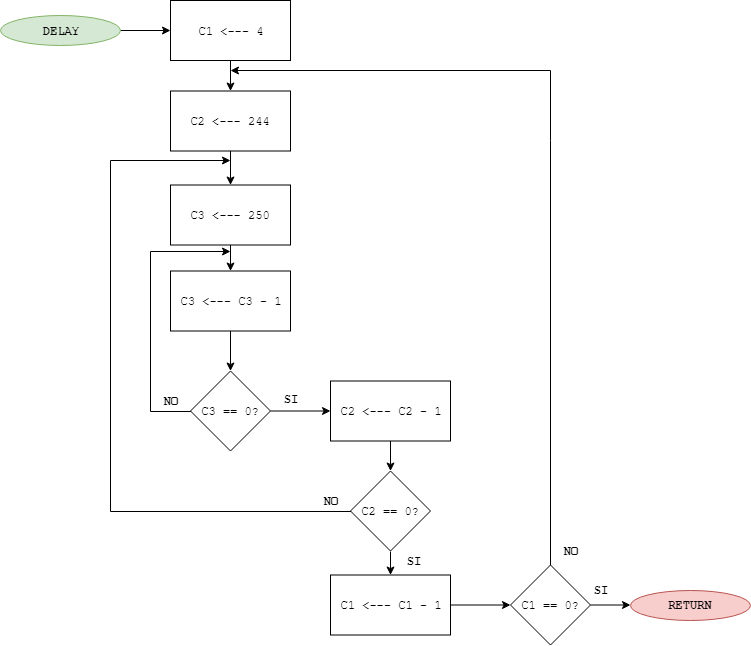
\includegraphics[scale=0.5]{delay.png}
	\centering
	\caption{Diagrama de flujo de la subrutina \emph{Delay}.}
	\end{figure}		
	
\newpage
\section{Esquema del circuito}

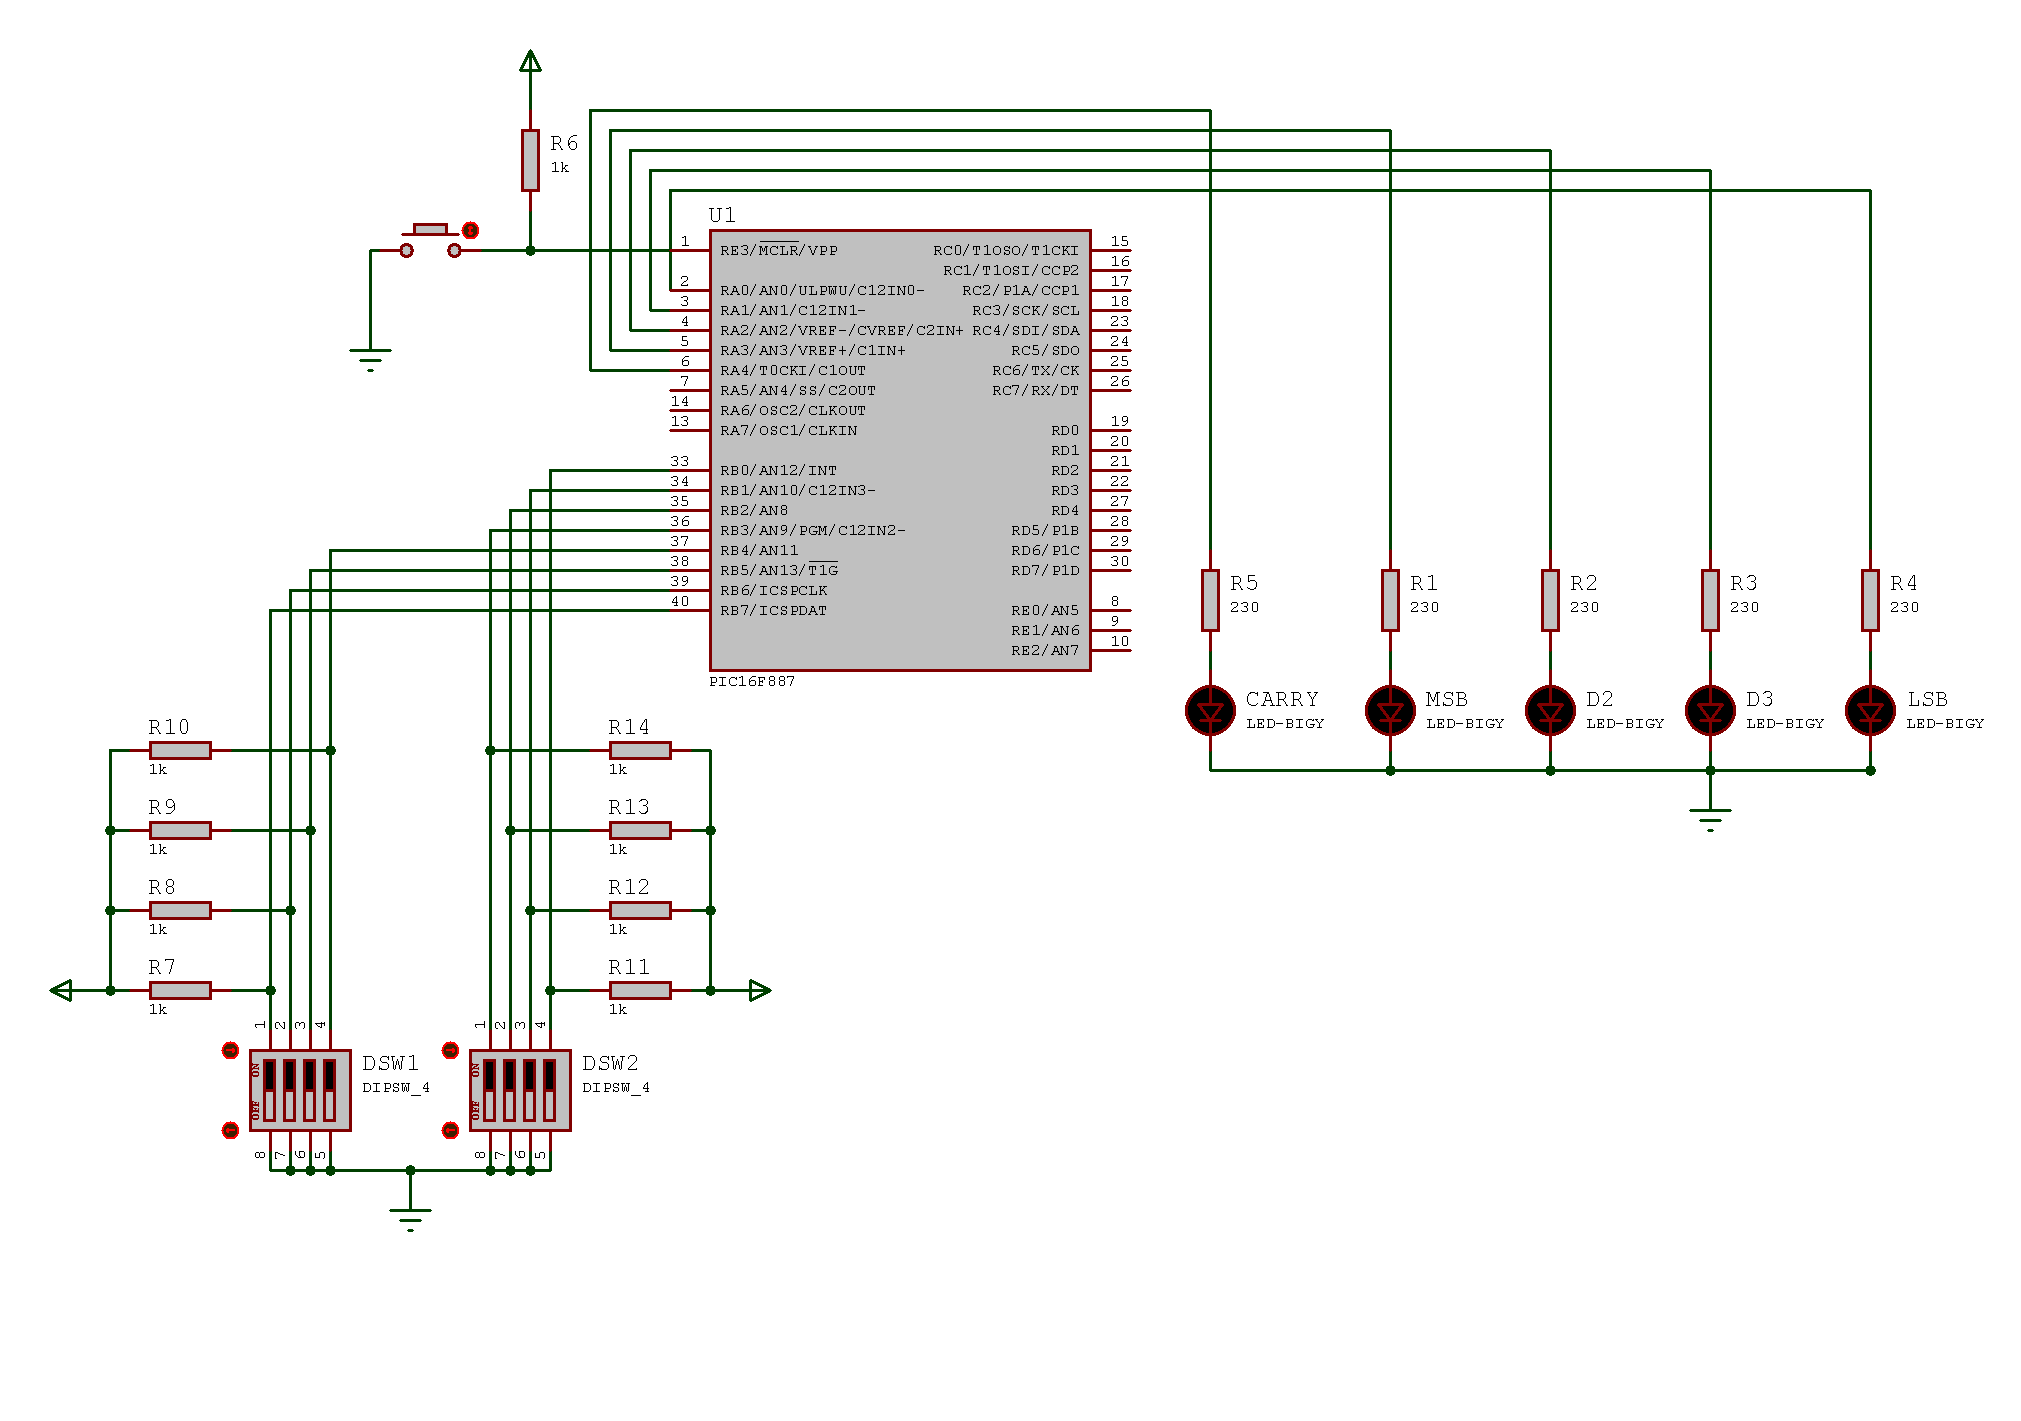
\includegraphics[angle=90,origin=c,scale=0.33]{circuito.png}
	
\end{document}